\subsection{Modellazione dati}
L'erogazione dei servizi da parte della API web necessità di una memorizzazione permanente di dati, incapsulati all'interno di entità.

Nel dettaglio si hanno:
\begin{itemize}
    \itemsep0em
    \item User: incapsula le informazioni dell'utente.
    \item Auth Mail: utilizzata per tenere traccia delle email di verifica dell'account e recupero della password.
    \item User Identity: rappresenta un'identità di terze parti.
    \item Refresh Token: rappresenta il refresh token di proprietà di un utente.
    \item Demo Subscription: identifica una sottoscrizione a un servizio demo da parte di un utente.
\end{itemize}

\newpage
\begin{figure}[h]
    \centering
    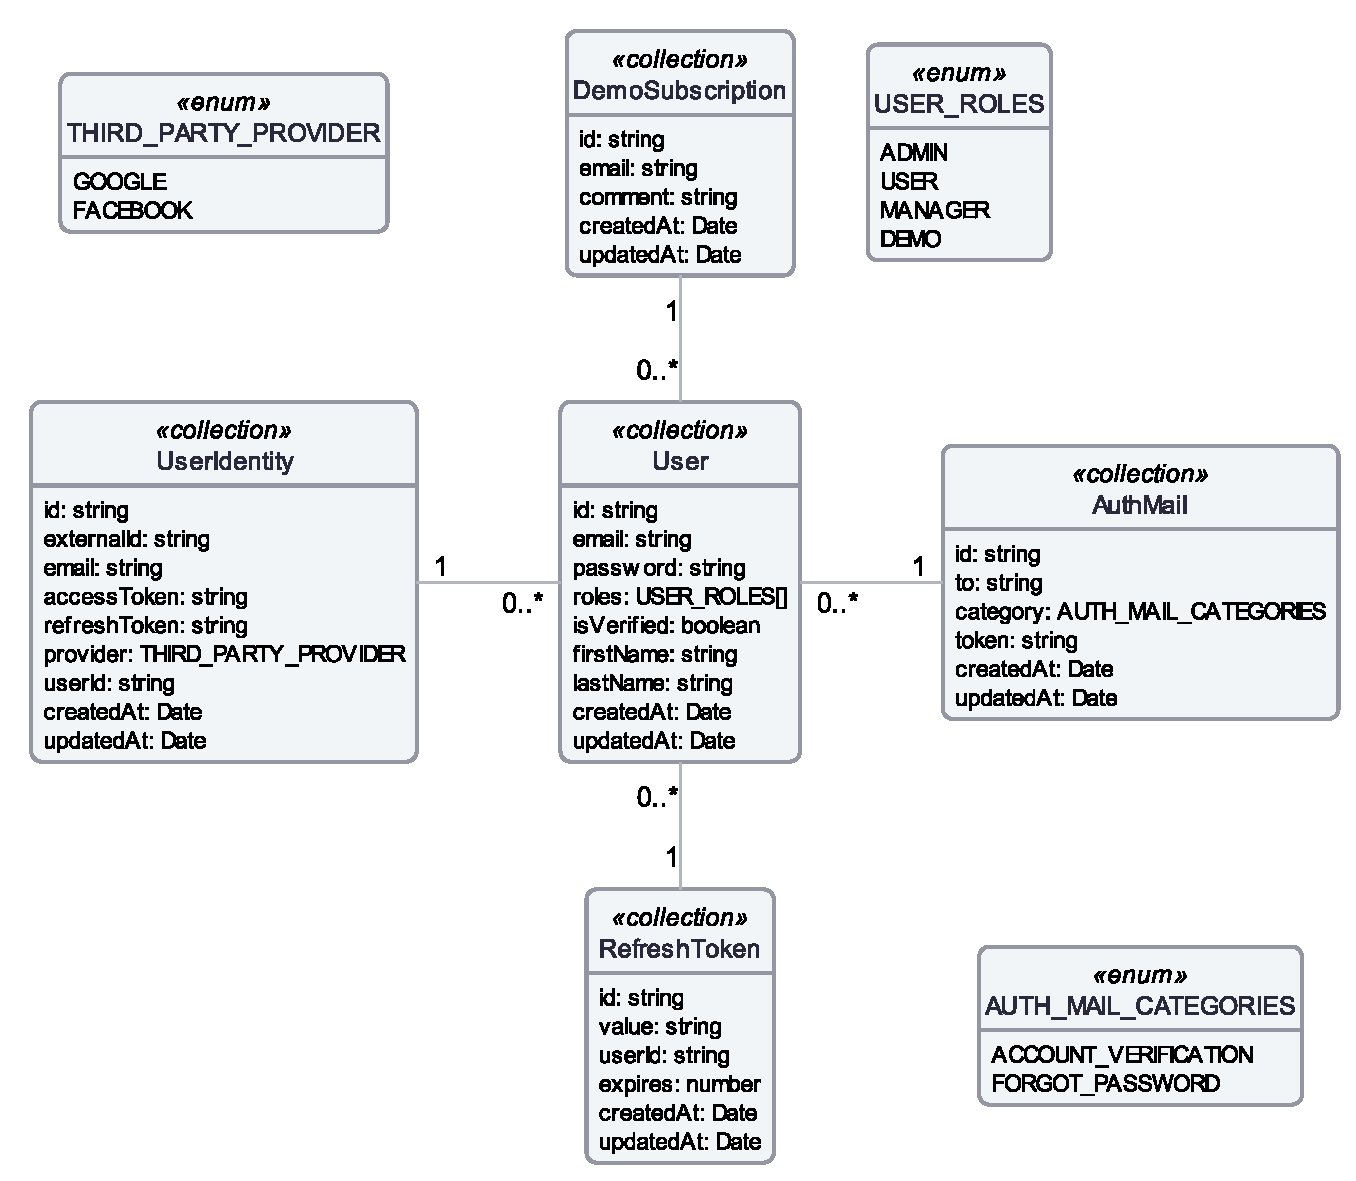
\includegraphics[width=0.90\textwidth]{data-model.eps}
    \caption{Modellazione dati}
    \label{fig:DataModel}
\end{figure}

Per l'implementazione è stato deciso di utilizzare MongoDB, un database non relazionale basato su documenti.
Per interfacciarsi con esso è stato deciso di utilizzare Typegoose\cite{Typegoose}: una libreria \textit{Object Data Modelling} (ODM) per gestire le relazioni tra i dati,
validare gli schemi e convertire il formato delle informazioni usato nel codice e nel database; tutto ciò con la possibilità di sfruttare la tipizzazione tipica di Typescript.
